\documentclass{beamer}
\DeclareFontShape{OT1}{cmss}{b}{n}{<->ssub * cmss/bx/n}{} 
\usetheme{default}
\usepackage{amsmath}
\usepackage{xcolor} % before tikz or tkz-euclide if necessary
\usepackage{tkz-euclide} % no need to load TikZ
\usepackage{multirow}

\title{Statistical Machine Learning\\ Part 2}
\author{Horacio G\'omez-Acevedo\\ Department of Biomedical Informatics}
\begin{document}
	\begin{frame}[plain]
		\maketitle
	\end{frame}
	\begin{frame}{Linear Discriminant Functions}
		A real-valued  function such as 
	
		\begin{equation}
			g(\mathbf{x})=\mathbf{w}^t \mathbf{x} +w_0	
			\label{eq:disc}
	\end{equation}	
	is called a {\bf discriminant function},
	where $\mathbf{w}$ is refer to as {\bf weight vector}, and  $w_0$  is normally called {\bf bias} (not the same as the statistical term). 
	
	For the discriminant function (\ref{eq:disc}) , we can define a two-category classifier (with classes $w_1$ and $w_2$) with the following rule:
	\begin{itemize}
		\item $\mathbf{x}\in w_1$ if $g(\mathbf{x}) >0$,
		\item $\mathbf{x}\in w_2$ if $g(\mathbf{x}) <0$
		\item if $g(\mathbf{x})=0$, then $\mathbf{x}$ can be assigned to either class.
	\end{itemize}
\end{frame}

\begin{frame}{Geometry related to the discriminant function}
	The equation $g(\mathbf{x})=0$ describes the {\bf decision surface} that separates both categories. If $\mathbf{x}_1$ and $\mathbf{x}_2$ are in the decision surface
	\begin{equation*}
		\mathbf{w}^t \mathbf{x}_1+w_0= \mathbf{w}^t \mathbf{x}_2+ w_0 \Rightarrow \mathbf{w}^t (\mathbf{x}_1 - \mathbf{x}_2)=0
	\end{equation*}
This implies that the vector $\mathbf{w}$ is normal to the hyperplane $H$ defined (generated) by the decision surface.
We can represent 
\begin{equation*}
	\mathbf{x}= \mathbf{x}_p+ r \frac{\mathbf{w}}{||\mathbf{w}||}
\end{equation*}
where $\mathbf{x}_p$ is the normal projection of $\mathbf{x}$ onto $H$ and $r$ is a signed distance (the sign depends on the side of the point $\mathbf{x}$ with respect to the separating plane $H$). More specifically,
\begin{equation*}
	r= \frac{g(\mathbf{x})}{||\mathbf{w}||}
\end{equation*}
\end{frame}

\begin{frame}{Confusion Matrix}
	A binary classifier placing instances in two classes $w_1$ and $w_2$ can make two types of error:
	\begin{itemize}
		\item it can assign an instance of $w_1$ into $w_2$
		\item it can assign an instance of $w_2$ into $w_1$
	\end{itemize}
The {\bf confusion matrix} allows us to summarize this information by putting it into a matrix in which each row represents the {\it actual} class, and each column represents the {\it predicted} class.

\begin{figure}
	\centering
	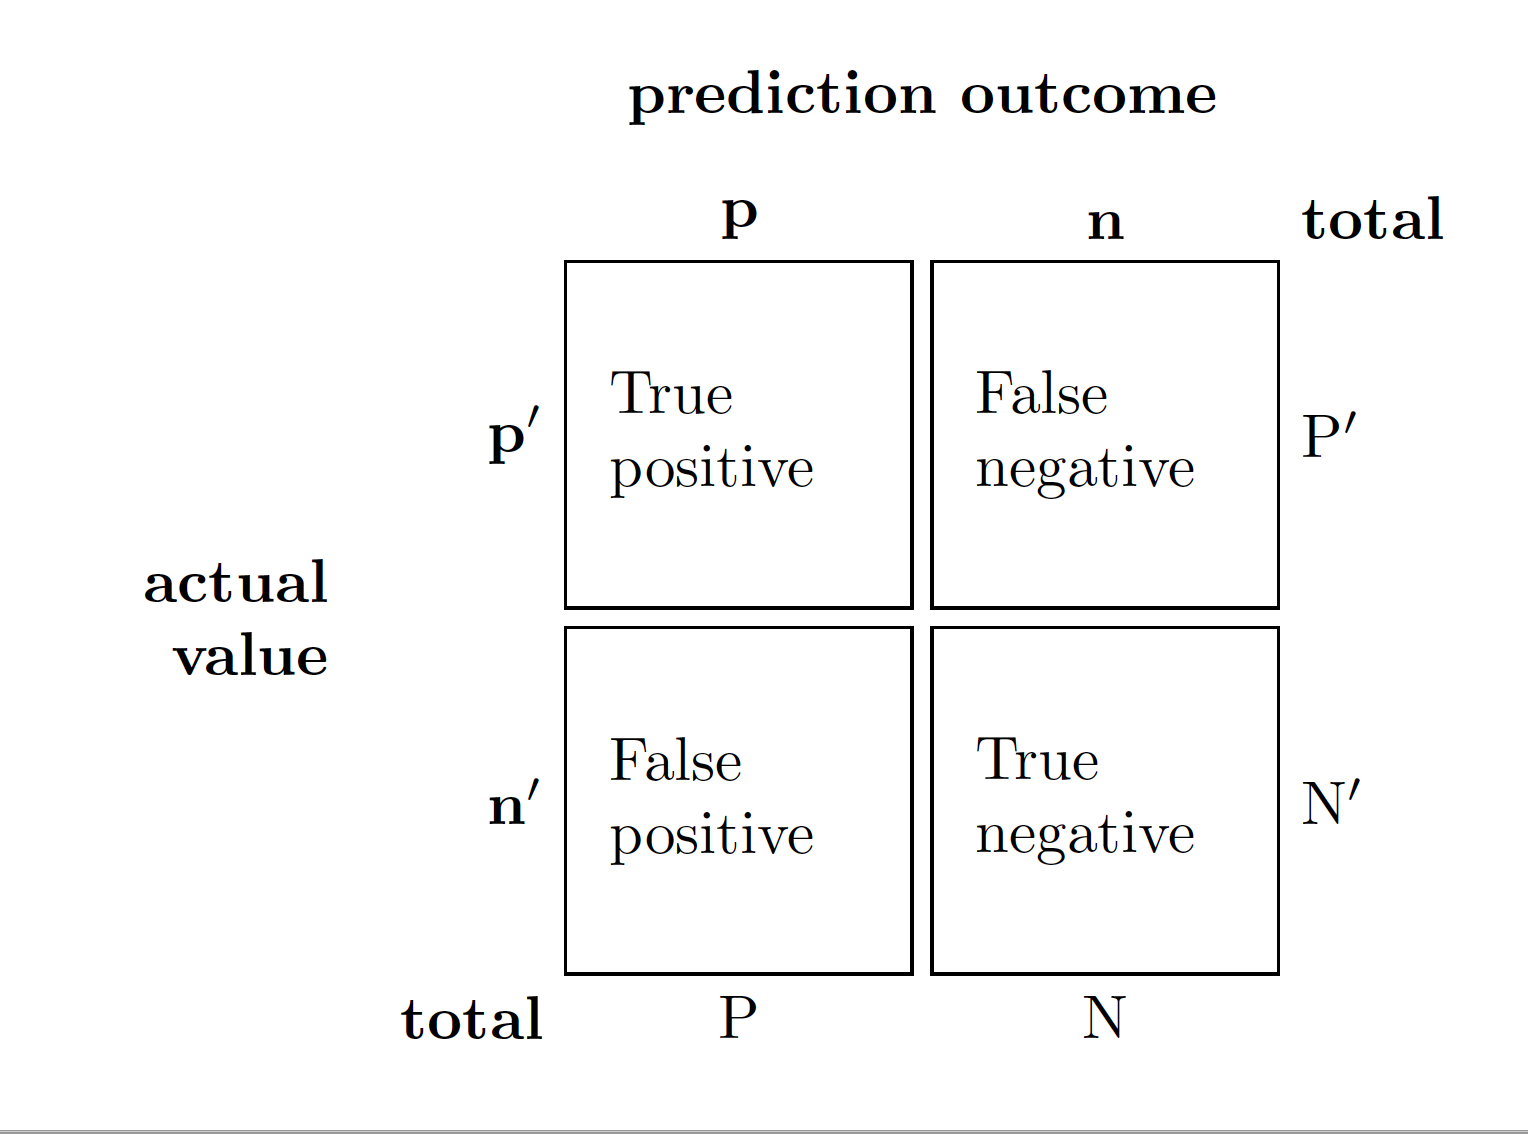
\includegraphics[scale=0.25]{../../Figures/fig_confusionmatrix.png}
\end{figure}

\end{frame}

\begin{frame}{Useful metrics}
	Once you have developed your binary classifier there are some common metrics to determine how well your classifier works.
	
	{\bf Precision} is defined as
	\begin{equation*}
		\textrm{precision}= \frac{TP}{TP+FP}
	\end{equation*}
	and the {\bf recall}  defined by the following expression
	\begin{equation*}
		\textrm{recall}= \frac{TP}{TP+FN}
	\end{equation*}
We also use another metric called the $F_1$ score that represents the harmonic mean of the precision and recall. 
\begin{equation*}
F_1= \frac{1}{\frac{1}{2}( \frac{1}{\textrm{precision}}+ \frac{1}{\textrm{recall}})}=\frac{TP}{TP+ \frac{FN+FP}{2}}
\end{equation*}
\end{frame}	

\begin{frame}{Observations about classifier metrics}
	\begin{itemize}
		\item False positives are  also known as {\it false alarm} or type I error.
		\item False negative are also known as {\it miss} or type II error.
		\item Recall is also referred to as {\it sensitivity} or {\it hit rate}.
		\item Precision is also called {\it positive predictive value}.
		\item In theory, you would like that precision and recall to be equal to 1. But this is not possible due to the {\bf precision-recall tradeoff}. 
	\end{itemize}


Suppose you are developing a new molecular technique (algorithm) to detect certain type of cancer  

{\bf Silly Scenario 1 }
You have tested your tool in vitro. You would like to detect as few false positives samples as possible, thus your precision must be very high while sacrificing recall.

{\bf Silly Scenario 2.}
If you proceed with human samples, 
a false positive can be financially costly due to the extra cost of further testing, but a false negative may cause harm to patients. Thus,  you would prefer higher recall sacrificing precision.
\end{frame}

\begin{frame}{Precision-Recall function}
	The so-called precision-recall function is obtained when we change the bias in our discriminant function and calculate the precision and recall. 
\begin{figure}
	\centering
	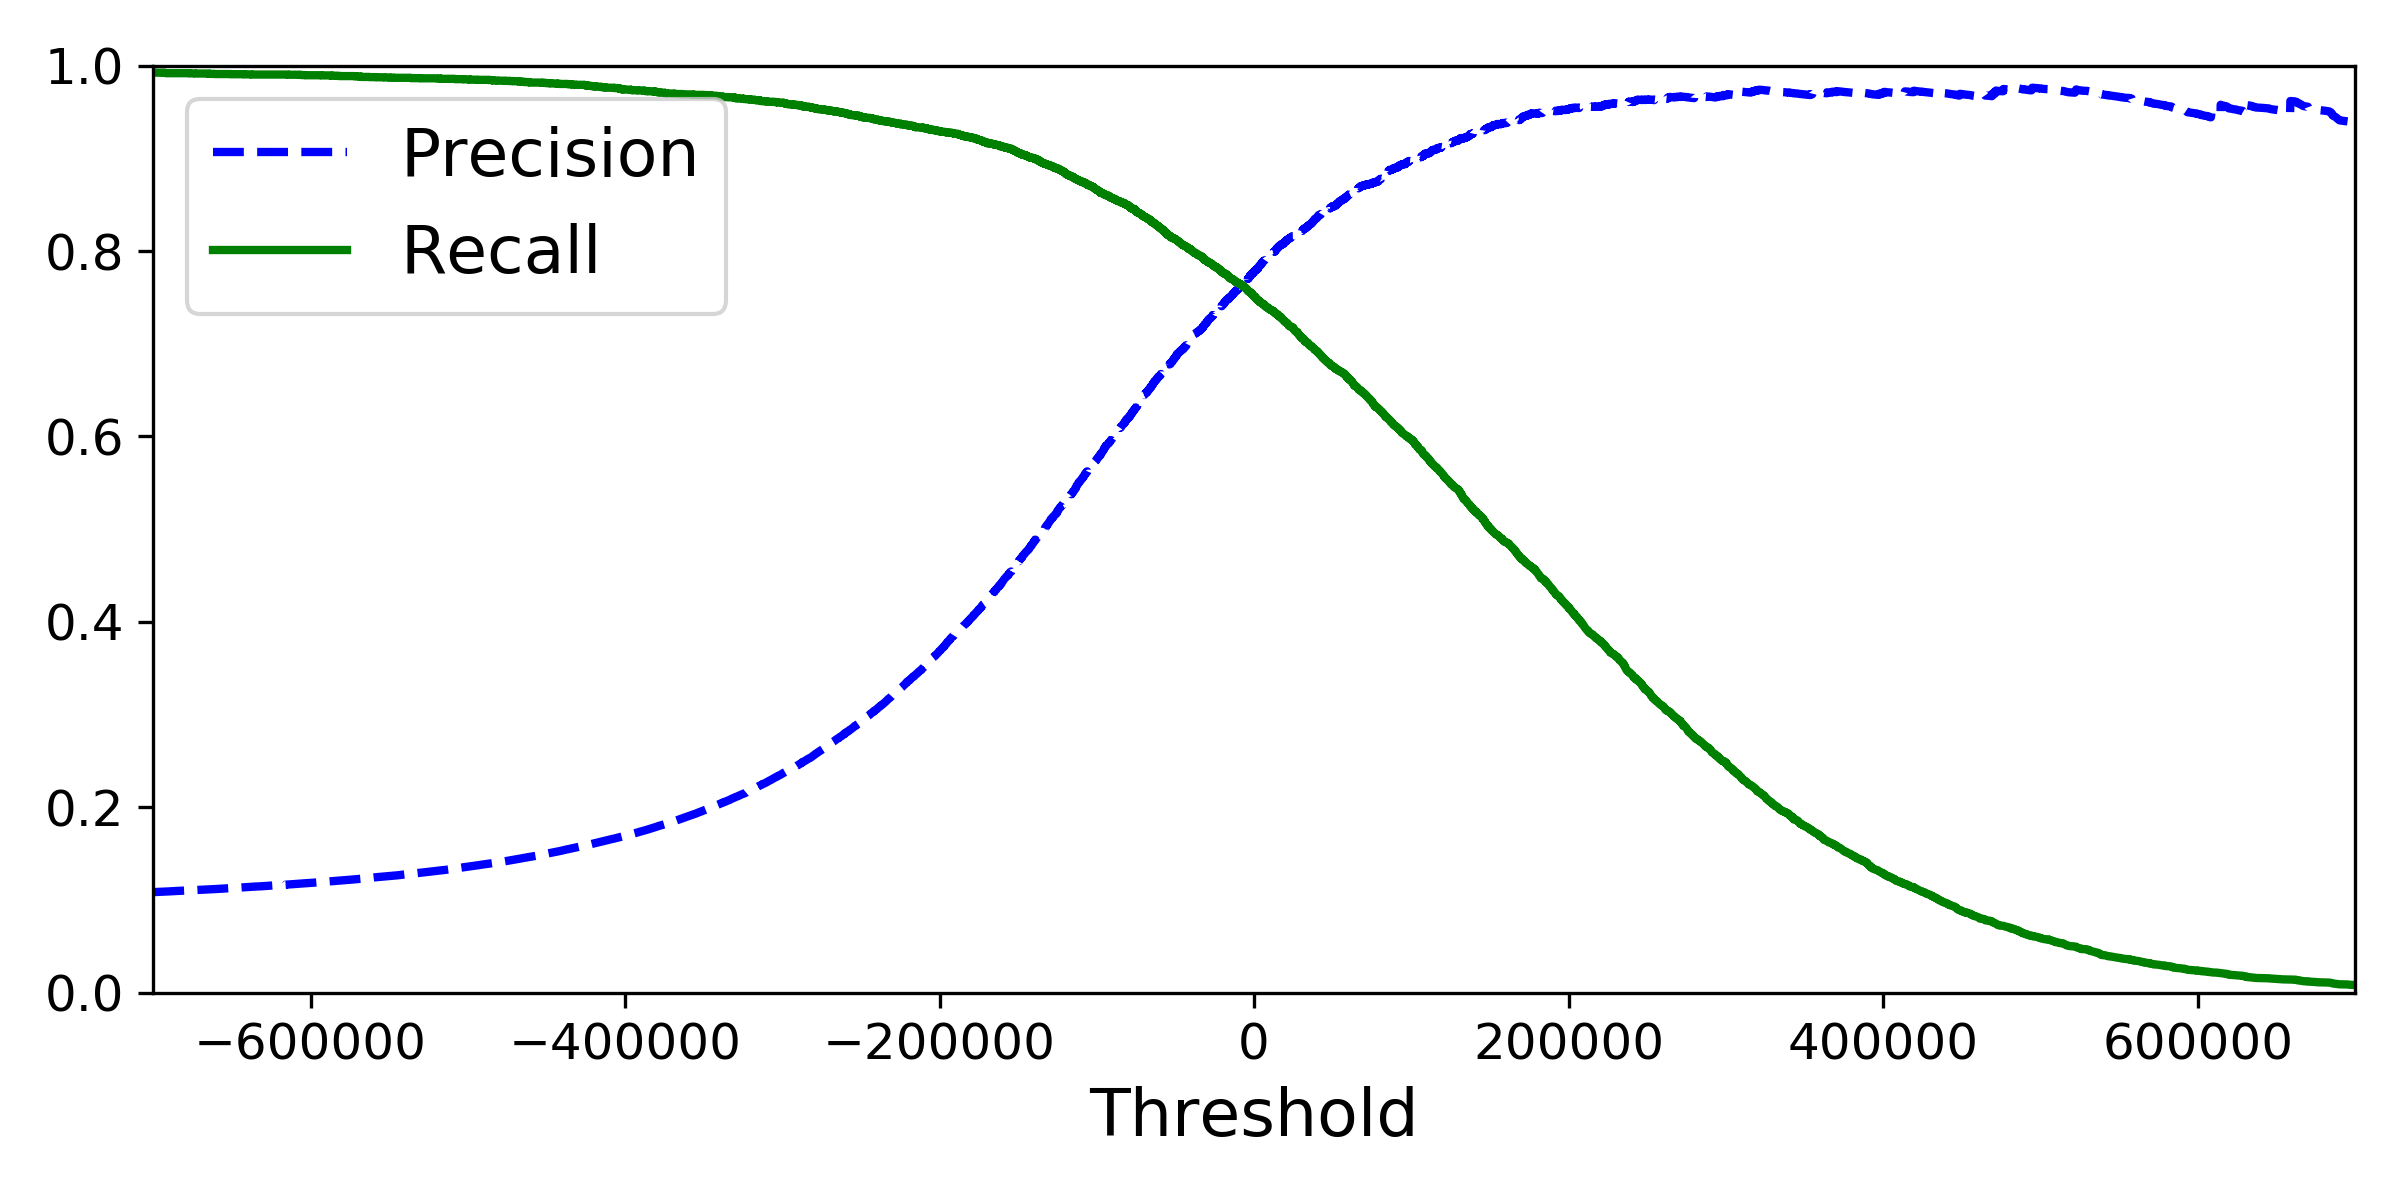
\includegraphics[scale=0.45]{../../Figures/precision_recall_vs_threshold_plot.png}
\end{figure}	
	
\end{frame}

\begin{frame}{ROC curve}
	The {\bf receiver operating characteristic curve (ROC)} plots the recall (true positive rate) against the {\it false positive rate}. 
	
	\begin{equation*}
		FPR= \frac{FP}{FP+TN}
	\end{equation*}
whereas the {\it true negative rate} or specificity 
\begin{equation*}
	TNR= \frac{TN}{FP+TN}
\end{equation*}
	Note that $FPR+TNR=1$, thus the ROC is a curve of the recall vs. 1-specificity, or FPR vs. TPR (if you want to keep everything positive!)
\end{frame}
\begin{frame}{ROC plot}
\begin{figure}
	\centering
	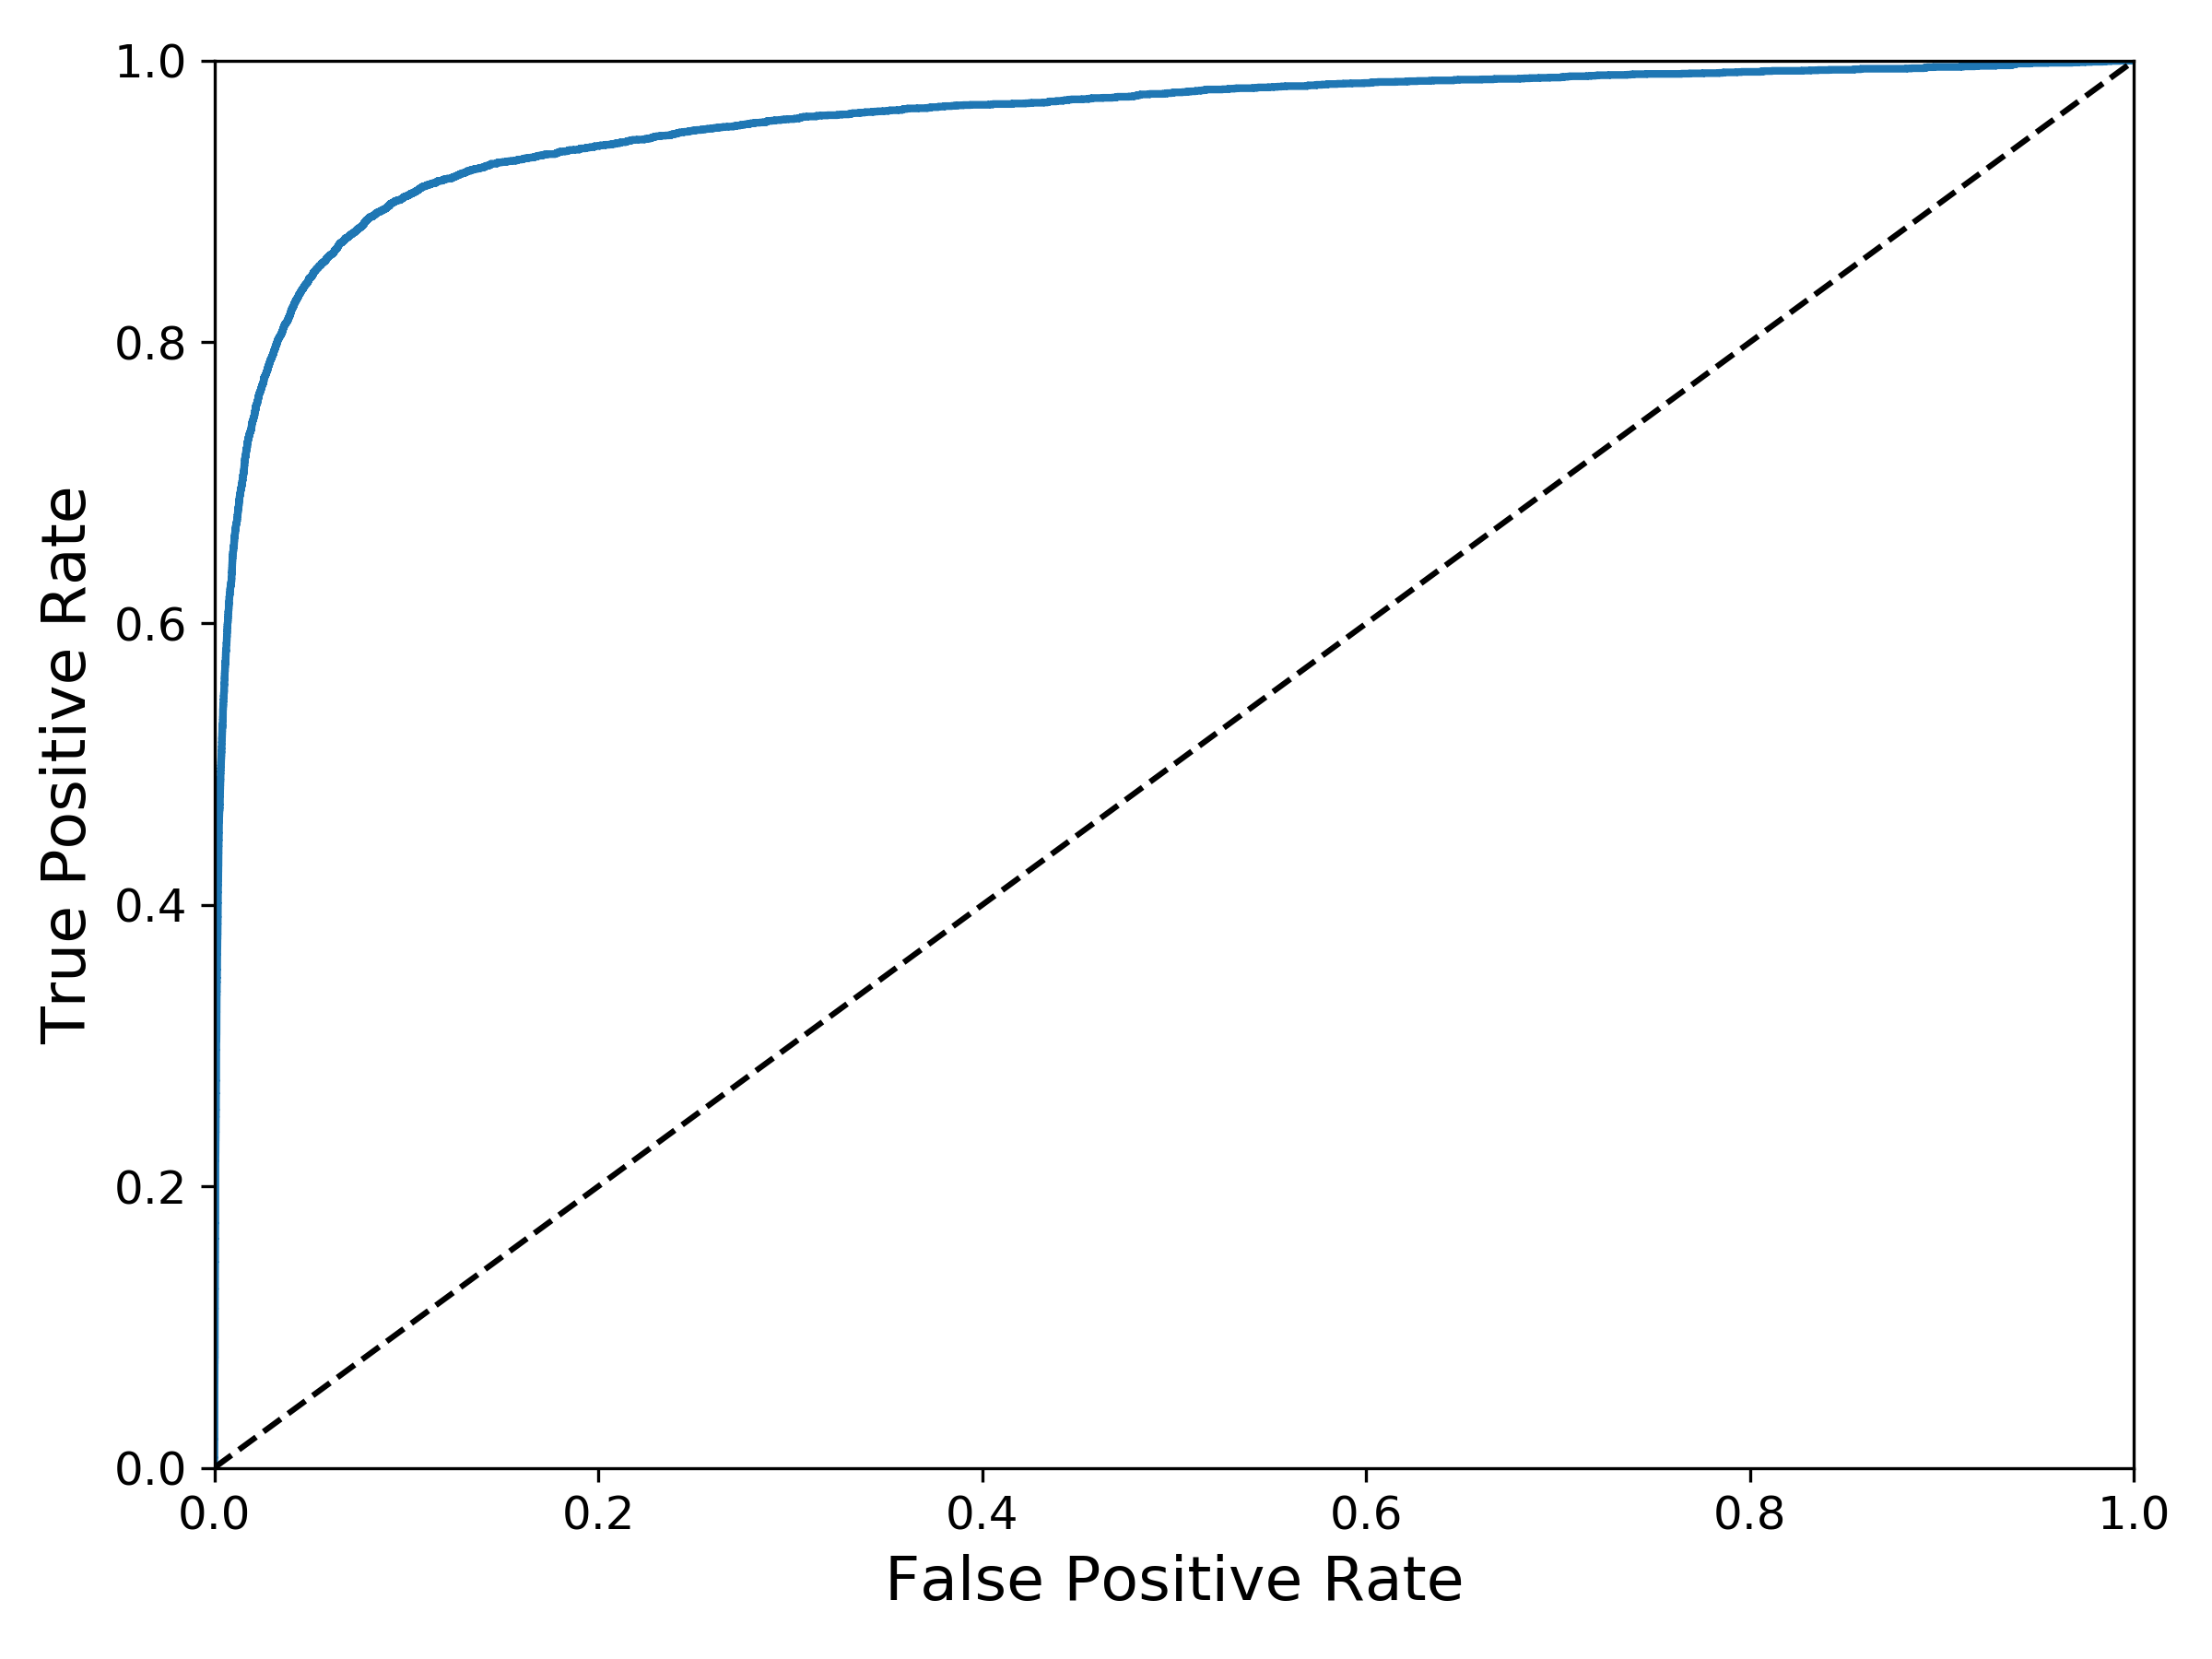
\includegraphics[scale=0.35]{../../Figures/roc_curve_plot.png}
\end{figure}
Normally, we calculate the "Area under the ROC curve" (AUROC) to compare our classification methods.

{\bf Note} If you have AUROC=0.5 your classifier is not doing better than a random choice.
\end{frame}


\end{document}